\chapter{Script Gadgets}
In this chapter, we present a novel XSS attack\todo{check others' work on how they introduce a main idea presented in the paper\\and structuring} (change this phrase) I will show how injecting benign HTML markup in a web page can also result in arbitrary JavaScript execution. The idea of the attack is based on abusing an already existed and trusted piece of JavaScript code (Script Gadget). 

\section{Modern Web Application}

JavaScript (JS) is \textit{the language of the web}. It’s a technology that was introduced to build dynamic web applications aiming for a richer web experience. All modern web applications contain JS code, which fundamentally interacts with other HTML elements (DOM elements)\todo{cite} to deliver that dynamism. Listing \ref{lst:modern_web} shows an arbitrary code snippet that is utilizing the \verb|data-*| attributes API defined in jQuery Mobile JavaScript library \cite{paper}. In brief, the code defines a UI element (a button) and an accompanying JavaScript code which uses a jQuery selector for reaching every UI element whose \verb|data-role| attribute value equals "button". The code then iterates over each button widget, extracting the value of its \verb|data-text| attribute and assign it as an inner content for the \verb|<button>| tag:
\\
\lstinputlisting[language=HTML,label={lst:modern_web},caption= A code snippet in a jQuery Mobile Web App]{listings/modern_web_1.html}

\section{Code-reuse attack and Script Gadgets}

It worth mentioning that, although the code in listing 1 was written for particular context (jQuery Mobile application), it, however, expresses a generic code pattern that is common in most modern JavaScript libraries or even user-land code. From the point of view of XSS Mitigations, injecting new HTML markup similar to the \verb|<div>| element in linting \ref{lst:modern_web} will be fine, at the end it doesn’t contain any code execution markup like \verb|<script>| tag nor inline event handlers like \verb|onclick=””| which usually make a particular injected payload suspicious for most mitigations. Consequently, we call that \verb|<div>| markup a Benign HTML markup. 

Now thinking of a new scenario, if there was a possibility to inject an arbitrary HTML markup one can inject a markup similar to on in listing \ref{lst:moderb_web_attack}:
\\
\lstinputlisting[language=HTML,caption=tbd,label={lst:moderb_web_attack}]{listings/modern_web_2.html}

Although the injected markup is a normal HTML div element, it’s obvious that the value of its data-text attribute now contains an attacker-controlled script input. Nevertheless, most mitigation techniques will report that markup as benign and safe to be part of the DOM, considering that the payload inside data-text attribute is a normal String. Injecting this div markup in its own will not result in any JS execution; however, since the value of its data-role attribute is also button and hence matches the DOM selector of the accompanying JS code, the injection will trigger that legitimate JavaScript code in the web page for execution. As a result, the script code defined in data-text attribute tag will be extracted and then injected to be part of the DOM resulting in execution of the attacker-controlled input script or XSS as shown in following:

\verb|<div data-role="button" ... ><script>alert(1)</script></div>|

The accompanying JS code mentioned in the example is called a \textit{Script Gadget}. Script Gadget is defined as piece of trusted JS already defined as part of the application code base and is triggered because of a benign HTML markup injection matches its selectors. 

XSS attacker can abuse Script Gadget\footnotemark and perform a code-reuse attack by injecting HTML markup (Need to be checked) with They convert otherwise safe HTML markup and attributes into arbitrary JS code execution. As illustrated in Figure 1.


\footnotetext{http://underscorejs.org/\#template}

\section{Attack Summary}

\begin{figure}
	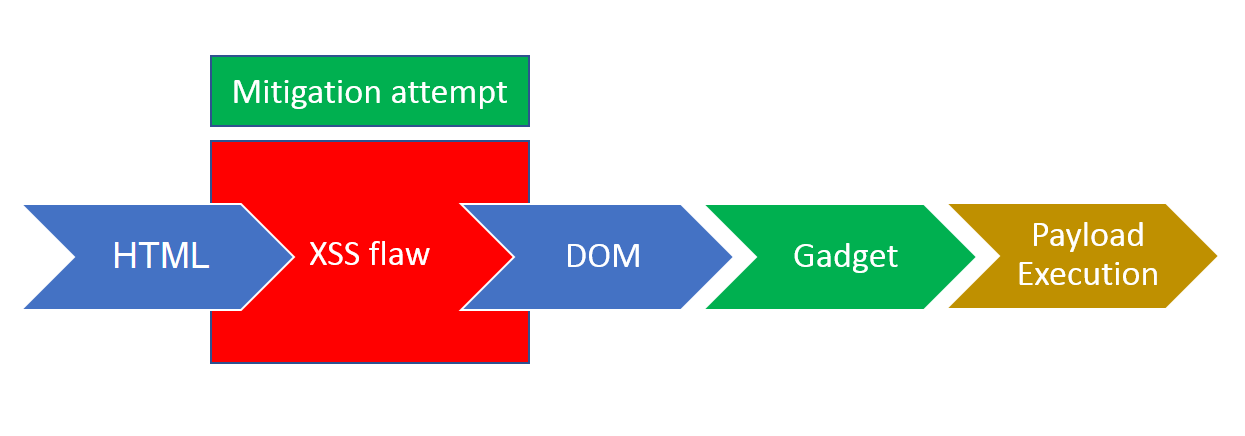
\includegraphics[width=\linewidth]{figures/attack_outline}
	\caption{Code-reuse attack outline}
	\label{fig:gadget_attack_outline}
\end{figure}

